\documentclass[russian]{beamer}
%\documentclass[handout]{beamer} %раздаточный материал
%\documentclass[aspectratio=169]{beamer}

%%% Работа с русским языком
\usepackage{cmap} %поиск в PDF
\usepackage{mathtext} %русские буквы в формулах
\usepackage[T2A]{fontenc} %кодировка
\usepackage[utf8]{inputenc} %кодировка исходного текста
\usepackage[english,russian]{babel} %локализация и переносы

%%Beamer по-русски
\newtheorem{rtheorem}{Теорема}
\newtheorem{rproof}{Доказательство}
\newtheorem{rexample}{Пример}

%%% Матпакеты
\usepackage{amsmath,amsfonts,amssymb,amsthm,mathtools} %AMS
\usepackage{icomma} %"Умная запятая": $0,2$ --  число, $0, 2$ -- перечисление

%% Номера формул
%\mathtoolsset{showonlyrefs=true} %Показывать номера только у тех в формул,
%на которые есть \eqref{} в тексте
%\usepackage{legno} %нумеризация формул слева

%%Свои команды
\DeclareMathOperator{\sgn}{\mathop{sgn}}

%%Перенос знаков в формулах (по Львовскому)
\newcommand*{\hm}[1]{#1\nobreak\discretionary{}
	{\hbox{$\mathsurround=0pt #1$}}{}}

%%%Работа с картинками
\usepackage{graphics} %Для вставки рисунков
\graphicspath{{images/}} %папки с картинками
\setlength\fboxsep{3pt} %отступ рамки \fbox{} от рисунка 
\setlength\fboxrule{1pt} %толщина линий рамки \fbox{}
\usepackage{wrapfig} %обтекание рисунков и таблиц текстом

%%%Работа с таблицами
\usepackage{array,tabularx,tabulary,booktabs} %дополнительная работа с таблицами
\usepackage{longtable} %длинные таблицы
\usepackage{multirow} %слияние строк в таблице

\usepackage{caption}

\usetheme{Montpellier} %тема оформления
%beamer theme matrix
\usecolortheme{crane}

%%%Заголовок
\author[]{Панчишин Д.И.
\and Носков Р.И.
\and Пасютин А.С.
}
\title[Презентация]{Проект \textbf{«\LaTeX»}}
\subtitle{Выполнили студенты 1 курса, ФИТ-204:}
\date[]{}
\institute[]{}

\begin{document}
	
	\begin{frame}
		\maketitle
	\end{frame}

\begin{frame}
	\frametitle{Цели}
	\begin{itemize}
		\item Научиться делать документы с высококачественной версткой текста и формул
		\item Продемонстрировать группе возможности \LaTeX'а
	\end{itemize}
\end{frame}

\begin{frame}
	\frametitle{Задачи}
	\begin{itemize}
		\item Изучение инструментов и макропакетов \TeX’а
		\item Получение навыков верстки текста в \LaTeX'е
		\item Создание отчета по проекту в системе \LaTeX
	\end{itemize}
\end{frame}

\begin{frame}
	\frametitle{Индивидуальные задачи}
	\begin{enumerate}
		\item<1-> \textbf{Панчишин Даниил} - Тим-лид, создание тех задания, работа в \LaTeX’е с мат. формулами, рисунками и графиками;
		\item<2-> \textbf{Носков Роман} - Работа в \LaTeX’е с инструментами для верстки текста;
		\item<3-> \textbf{Пасютин Александр} - Работа в \LaTeX’е с инструментами для работы с презентациями.
	\end{enumerate}
\end{frame}

\begin{frame}
	\frametitle{Календарный план}
	\begin{tabular}{|l|p{8cm}|}
		\hline
		18.02 & Распределение ролей, создание удаленного репозитория, составление календарного плана \\
		\hline
		4.03 & Изучение общего теоретического материала \\
		\hline
		18.03 & Начало работы над практической частью проекта \\
		\hline
		01.04 & Изучение отдельных аспектов \LaTeX’а, распределенных по ролям \\
		\hline
		15.04 & Создание презентации в \LaTeX, которая бы демонстрировала изученные навыки \\
		\hline
		29.04 & Создание отчета в \LaTeX, который бы демонстрировал изученные навыки
		\\
		\hline
		13.05 & Презентация результатов работы над проектом \\
		\hline
		27.05-31.05 & Защита проекта \\
		\hline
	\end{tabular}
\end{frame}

\begin{frame}
	\frametitle{Используемые средства}
\begin{figure}[h]
	\begin{center}
		\begin{minipage}[h]{0.4\linewidth}
			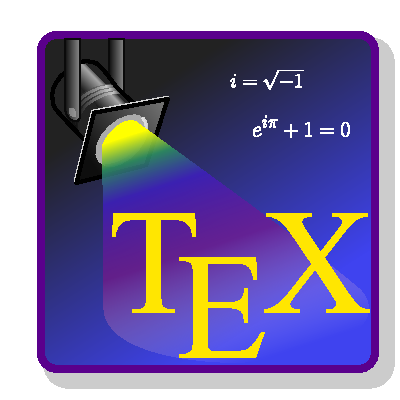
\includegraphics[width=5cm,height=5cm]{tex}
			\caption*{\huge{TeXStudio}}
		\end{minipage}
		\hfill											
		\begin{minipage}[h]{0.4\linewidth}
			
\includegraphics[width=5cm,height=5cm]{miktex}
			\caption*{\huge{MiKTeX}}
		\end{minipage}
	\end{center}
\end{figure}
\end{frame}

\begin{frame}
	\frametitle{Итоговый результат}
\end{frame}
\end{document}